\documentclass[aps, pre, onecolumn, a4paper, floatfix]{revtex4}
%\documentclass[twocolumn]{revtex4}
\usepackage{graphicx}
\usepackage{amsmath}
\usepackage{placeins}
\usepackage{color}
\usepackage{hyperref}
%\usepackage{bug}
%\bibliographystyle{plain}




\begin{document}

\title{Supplemental materials}
\author{Sebastian M. Krause}
\author{Vinko Zlati\'{c}}
\affiliation{Theoretical Physics Division, Rudjer Bo\v{s}kovi\'{c} Institute, Zagreb, Croatia}
\author{Michael M. Danziger}
\affiliation{Department of Physics, Bar Ilan University, Ramat Gan, Israel}
\begin{abstract}

\end{abstract}
%\pacs{89.65.-s, 05.50.+q, 05.65.+b, 64.60.De}
\maketitle

\section*{List of variables}
{\centering

\begin{tabular}{ c c }
 \hline
 \multicolumn{2}{ c } {Networks}\\
 \hline
 $N$ & Number of nodes \\
 $\bar k$ & Average degree \\
 $k_i$ & Degree of node $i$ \\
 $p_k$ & Degree distribution \\
 $\alpha$ & Exponent of scale free degree distribution \\
 $g_0$ & Generating function of degree \\
 $g_1$ & Generating function of excess degree \\
 \hline
 \multicolumn{2}{ c } {Colors}\\
 \hline
 $C$ & Number of colors \\
 $c\in 1,2,\dots C$ & A color \\
 $r_c$ & Color distribution \\
 $n_{\rm deg}$ & Degeneration of the highest color frequency \\
 ${\tilde r}_{c,k}$ & degree-dependent color distribution \\
 \hline
 \multicolumn{2}{ c } {Standard percolation ingredients}\\
 \hline
 ${\mathcal L}$ & Set of nodes in the largest component (color blind) \\
 $u$ & Prob.\ of not being connected to giant comp.\ over a link \\
 $S$ & Size of giant component \\
 $\phi_{\bar c}$ & Fraction of nodes without color $c$ \\
 ${\mathcal L}_{\bar c}$ & Set of nodes in the largest component, after nodes of color c deleted\\
 $u_{\bar c}$ & Prob.\ of not being connected to giant ${\mathcal L}_{\bar c}$ over a link \\
 $S_{\bar c}$ & Size of giant ${\mathcal L}_{\bar c}$ \\
 \hline
 \multicolumn{2}{ c } {Percolation over color avoiding paths}\\
 \hline
 ${\mathcal L}_{\rm color}$ & Candidate set of nodes for the largest avoidable colors component\\
 $S_{\rm color}$ & Size of giant ${\mathcal L}_{\rm color}$ \\
 $B_{k,k'}$ & Prob.\ that out of $k$ links $k'$ connect to giant component \\
 $M_{k',\vec \kappa}$ & Prob.\ that out of $k'$ links $\kappa_1$ connect to color 1 etc. \\
 $P_{\vec \kappa}$ & Success probability having neighbors of colors acc. to $\vec \kappa$ \\
 $U_{\bar c}$ & Prob.\ that a link fails connecting to ${\mathcal L}_{\rm color}$ which already connects to ${\mathcal L}$ and 
 a node not having color $c$\\
 $S_{{\rm color},\infty}$ & Size of the set of all nodes being connected to giant component over two links or more \\
 \hline
 \hline
 $\beta$ & Critical exponent \\
 ${\bar k}_{\rm crit}$ & Critical value of average degree \\
 $k_{\rm step}$ & Degree above which all nodes have the same color \\
 $\gamma$ & Fraction of nodes with highest degree \\
\end{tabular}

}



\pagebreak

\section{Size of giant avoidable colors component in the configuration model}

We can find analytical results for $S_{\rm color}$ for random graph ensembles 
with randomly distributed colors in the limit of infinite graphs. 
These results can be used to estimate the situation in finite quenched networks. 
We are able to gain a general understanding including phase transitions. 
This can guide our understanding of real world networks. 

We use the generalized configuration model graph ensemble with $N$ nodes, 
where each degree sequences $\{k_i\}$ occurs with probability $\prod_i p_{k_i}$, 
with the degree distribution $p_{k}$. 
Additionally we want to assign to every node $i$ a color $c_i\in 1,2,\dots,C$. 
For given degree sequence $k_i$, 
the color sequence $\{c_i\}$ has probability $\prod_i {\tilde r}_{c_i,k_i}$ 
with the degree-dependent color distribution ${\tilde r}_{c,k}$ 
($\sum_c {\tilde r}_{c,k}=1$ for every degree $k$ separately). 
For a graph $G_N$ out of the graph ensemble, 
$\mathcal{L}_{\rm color}$ has a certain size $N_{\rm color}(G_N)$. 
For the whole graph ensemble, we have to use the average value. 
By considering only giant contributions growing with network size, 
we have
\begin{align}
S_{\rm color} &= \lim_{N\to \infty}\sum_{G_N} P(G_N) \frac{N_{\rm color}(G_N)}{N},
\end{align}
where $P(G_N)=\prod_i p_{k_i} \omega \prod_i {\tilde r}_{c_i,k_i}$ is the probability 
to have the graph $G_N$ of size $N$, including $\omega$, 
the probability of the connection scheme of $G_N$ as a matching of half edges. 


\subsection{Question and connection to percolation theory}

For calculating $S_{\rm color}$ in the random graph ensemble, 
we will follow ideas of Erdos and Renij and Newman. 
For calculating the size of the giant component, 
they used probabilities of connections for a single node in the graph ensemble. 
As we have to extend the method to a gradual procedure with conditional probabilities, 
it is useful to introduce the original method in detail with a shifted viewpoint. 

\begin{figure}[htb]
  \begin{minipage}[b]{0.18\linewidth}
    \begin{center}
      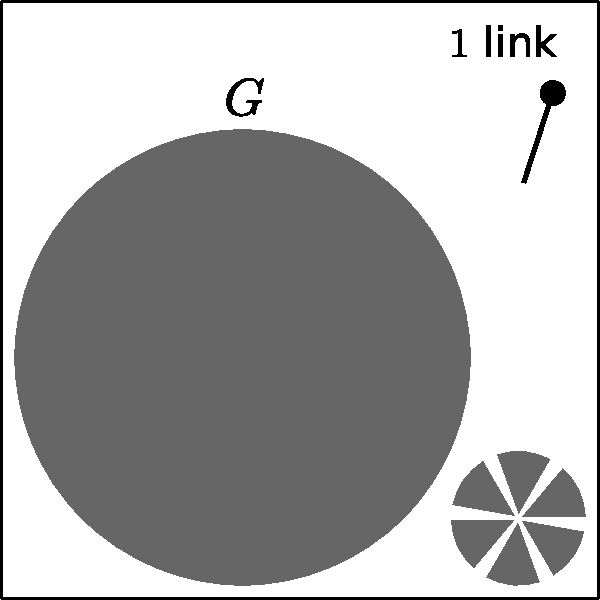
\includegraphics[width=0.99\columnwidth]{sets_gc_all1.pdf}
   \end{center}
  \end{minipage}
  \begin{minipage}[b]{0.05\linewidth}
    \begin{center}
      {\large $\xrightarrow{u}$}\\
      \vspace{15mm}
    \end{center}
  \end{minipage}
  \begin{minipage}[b]{0.18\linewidth}
    \begin{center}
      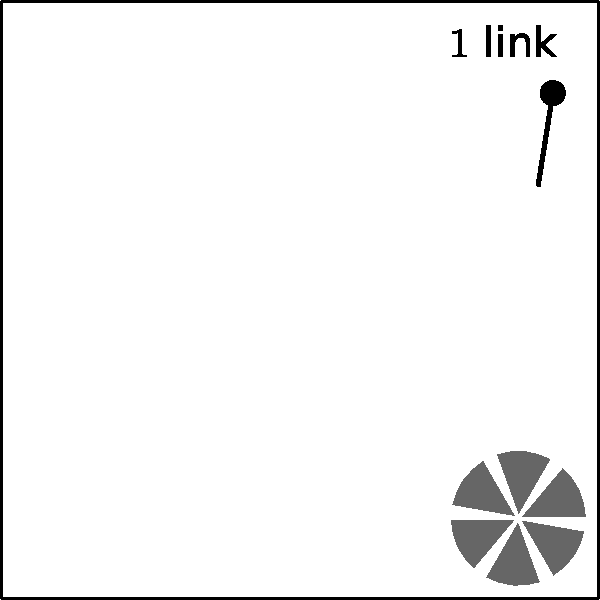
\includegraphics[width=0.99\columnwidth]{sets_gc_no1.pdf}
    \end{center}
  \end{minipage}
  \begin{minipage}[b]{0.05\linewidth}
  \ 
  \end{minipage}
  \begin{minipage}[b]{0.18\linewidth}
    \begin{center}
      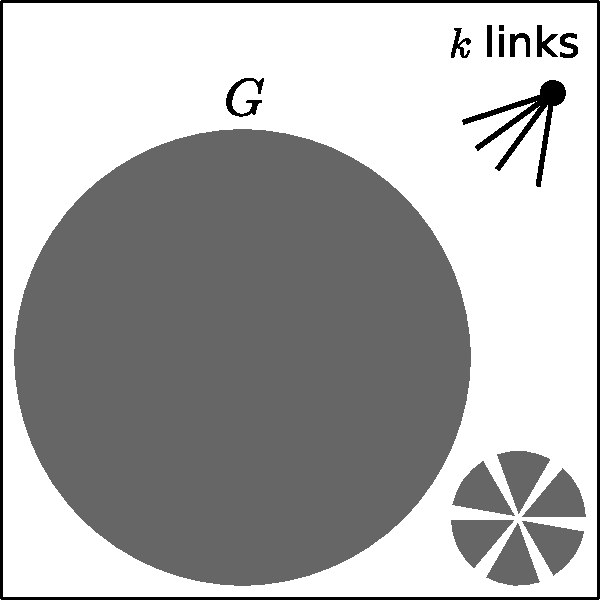
\includegraphics[width=0.99\columnwidth]{sets_gc_allk.pdf}
    \end{center}
  \end{minipage}
  \begin{minipage}[b]{0.07\linewidth}
    \begin{center}
      {\large $\xrightarrow{1-u^k}$}\\
      \vspace{15mm}
    \end{center}
  \end{minipage}
  \begin{minipage}[b]{0.18\linewidth}
    \begin{center}
      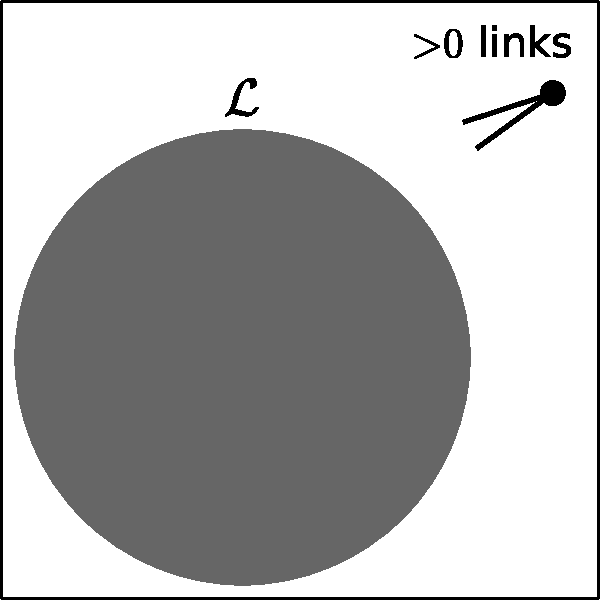
\includegraphics[width=0.99\columnwidth]{sets_gc_gck.pdf}
    \end{center}
  \end{minipage}
    \caption{We base our theory on the method to calculate the size of 
    normal giant components, as illustrated in this figure. Using a self 
    consistency equation, the probability $u$ can be calculated. This is the 
    probability, that a node is not connected to the giant component over a 
    single link (see on the left). On the right, the probability for a node 
    with $k$ links is illustrated to have at least one link connecting to 
    the giant component. $u^k$ is the probability that all links fail.}
    \label{fig:gc}
\end{figure}
%
Lets denote with $\mathcal{L}$ the set of all nodes belonging to the largest component. 
In figure~\ref{fig:gc} on the outer left, a possible situation is illustrated. 
The largest component contains of a large part of the network, 
and the remaining nodes belong to smaller components. 
We have to calculate the size $S$ of the giant component, 
meaning the average relative size of $\mathcal{L}$ in the network ensemble 
in the limit of infinite network size. 
For this we can define the average probability $u$ 
that a node fails to connect to $\mathcal{L}$ over one particular link.  
This is illustrated in the figure with the left part. 
Again, the thermodynamic limit $N\to \infty$ is implied. 
With the definition of $u$ at hand, we can calculate $S$ in two steps: 
First, using a self consistency equation, $u$ is calculated. 
The probability $u$ is identical to the probability 
that the neighbor does not connect to the giant component over any of the remaining links, 
\begin{align}
u &= g_1(u),\quad g_1(z)=\sum_k q_k z^k.\label{eq:u}
\end{align}
In this equation, $g_1$ is the generating function 
of excess degree $q_k=(k+1)p_{k+1}/\bar{k}$. 
For important degree distributions as e.g. Poisson or scale-free, 
the equation for $u$ can only be solved numerically. 
The second step is an averaging over nodes with various degrees $k$. 
The probability to connect to the giant component over any of $k$ links is $(1-u^k)$, 
meaning that not all links fail at the same time. 
This is illustrated in the figure on the right. 
As a node which connects to the giant component belongs to it, 
%%%
\begin{align}
S &= \sum_{k=0}^{\infty}p_k (1-u^k) = 1-g_0(u),\quad g_0(z)=\sum_k p_k z^k.\label{eq:S}
\end{align}

\begin{figure}[htb]
  \begin{minipage}[b]{0.245\linewidth}
    \begin{center}
    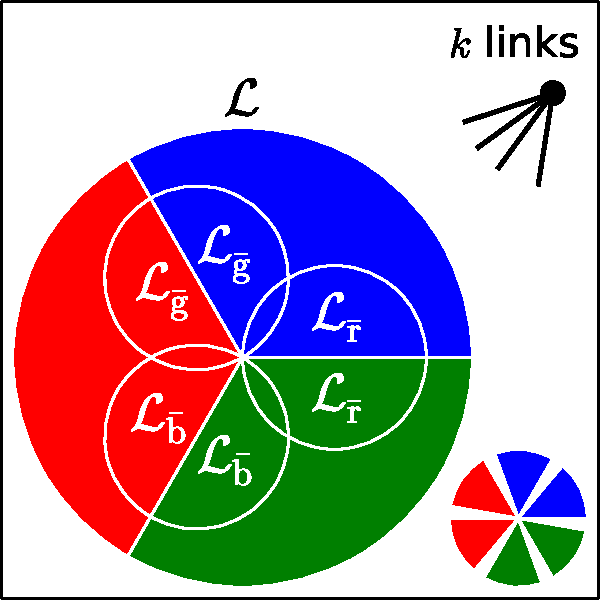
\includegraphics[width=0.99\columnwidth]{sets_k_all.pdf}
   \end{center}
  \end{minipage}
  \begin{minipage}[b]{0.1\linewidth}
    \begin{center}
      {\Large $\xrightarrow{?}$}\\
      \vspace{20mm}
    \end{center}
  \end{minipage}
  \begin{minipage}[b]{0.6\linewidth}
    \begin{center}
    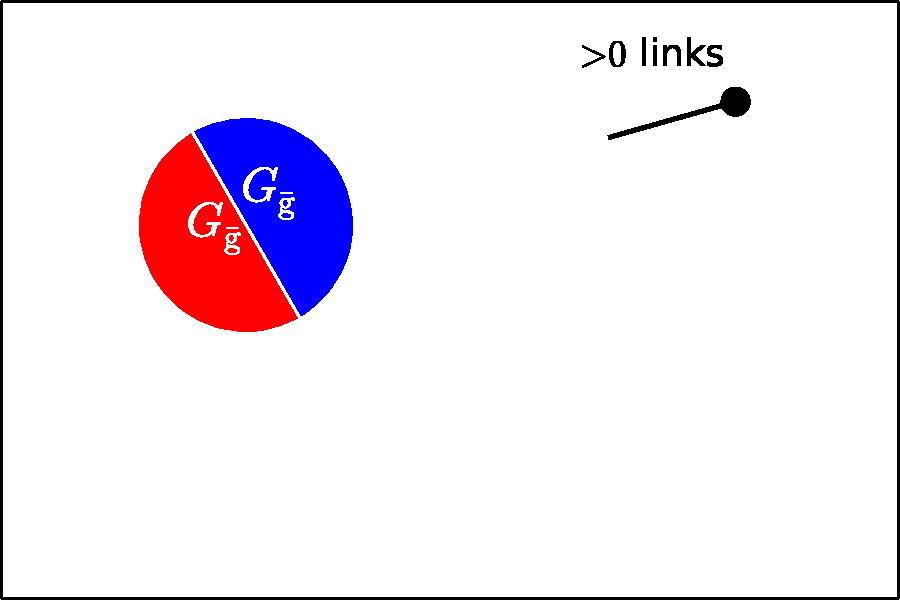
\includegraphics[height=0.4\columnwidth]{sets_k_gc_no_2.pdf}
     \hspace{-1mm}
    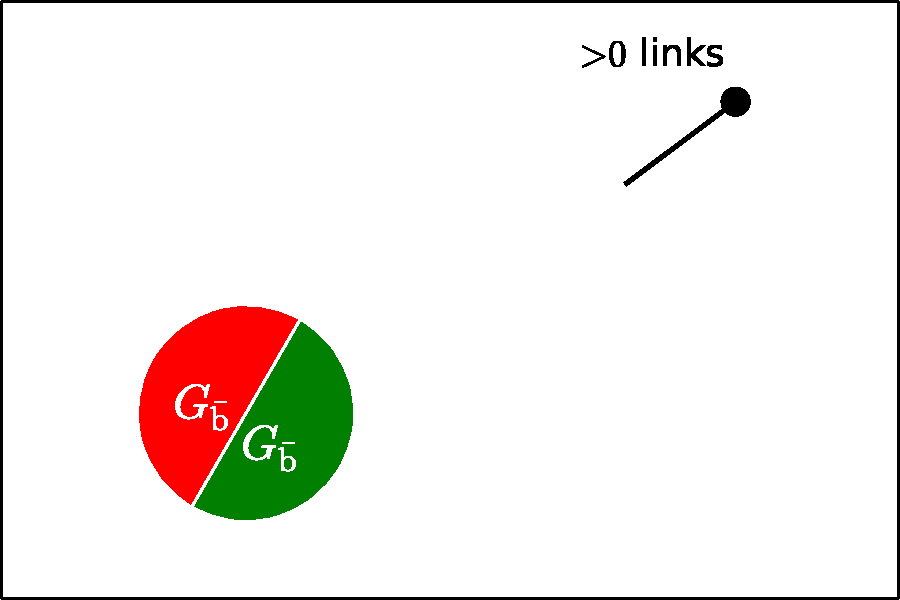
\includegraphics[trim=100 0 0 0,clip,height=0.4\columnwidth]{sets_k_gc_no_3.pdf}
     \hspace{-1mm}
    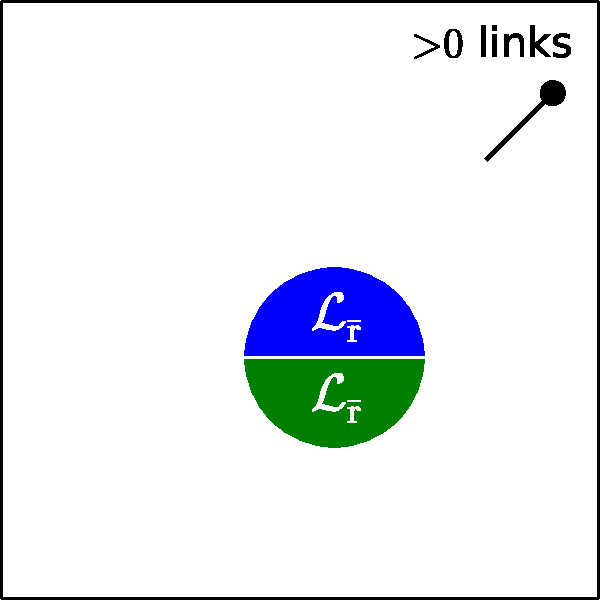
\includegraphics[trim=100 0 0 0,clip,height=0.4\columnwidth]{sets_k_gc_no_1.pdf}
   \end{center}
  \end{minipage}
    \caption{We have to calculate the probability, if a node with $k$ links is 
    for every color $c$ connected to the giant component $\mathcal{L}_{\bar c}$ with deleted 
    color $c$. All connections over at least one link have to exist at the same 
    time. We illustrate this question with the three colors red ($c=$r), green 
    ($c=$g) and blue ($c=$b). If a link connects to $\mathcal{L}_{\bar{\rm g}}$, it for 
    sure does not connect to $\mathcal{L}_{\bar c}$ for one of the other colors. This kind of 
    dependence forces us to use a stepwise calculation with conditional probabilities.}
    \label{fig:question}
\end{figure}

In analogy to the procedure described above, 
we will calculate $S_{\rm color}$ as the probability 
that a randomly chosen node belongs to $\mathcal{L}_{\rm color}$. 
This has to be evaluated in the graph ensemble of infinite size. 
As we will perform an averaging over nodes with various degrees $k$, 
the following question has to be answered: 
What is the probability that a node with $k$ links connects 
to a giant $\mathcal{L}_{\bar c}$ for all colors $c$ at the same time. 
This is illustrated in figure~\ref{fig:question}. 
On the left, the situation for a graph with colors on the nodes is illustrated. 
Nodes of all colors might be in the largest component. 
After deleting all nodes of one color $c$, 
the remaining largest component $\mathcal{L}_{\bar c}$ 
might still contain a large part of all nodes in $\mathcal{L}$. 
The condition for the node belonging to $\mathcal{L}_{\rm color}$ 
is illustrated on the right of the figure. 

We will use the same two steps to attack this problem, 
as described for calculating the giant component above. 
First, we provide some single link probabilities 
which can be used as primitives for the further calculations. 
Second, we combine the single link probabilities to calculate $S_{\rm color}$. 


\subsection{Single link probabilities}



\begin{figure}[htb]
   \begin{center}
    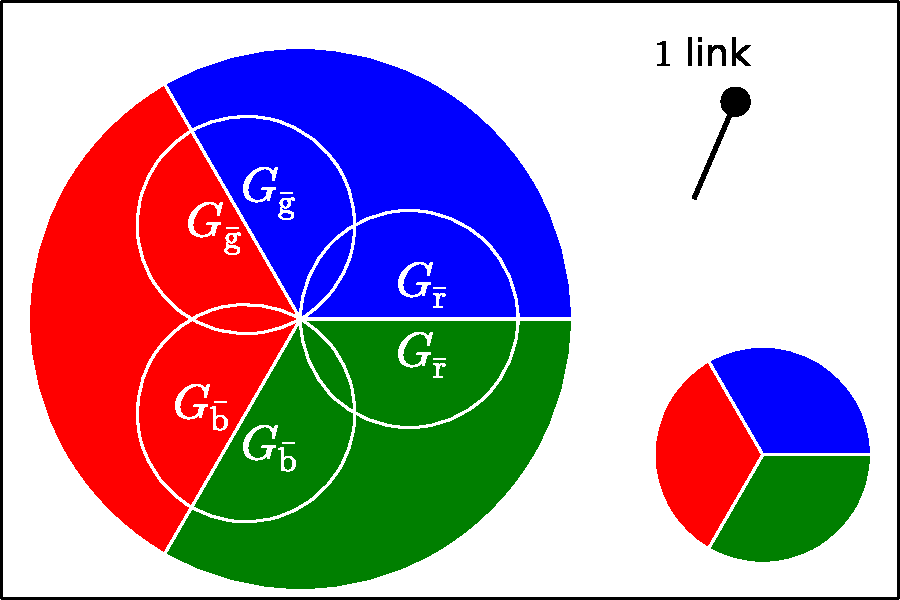
\includegraphics[width=0.2\columnwidth]{sets_1_all.pdf}\qquad
    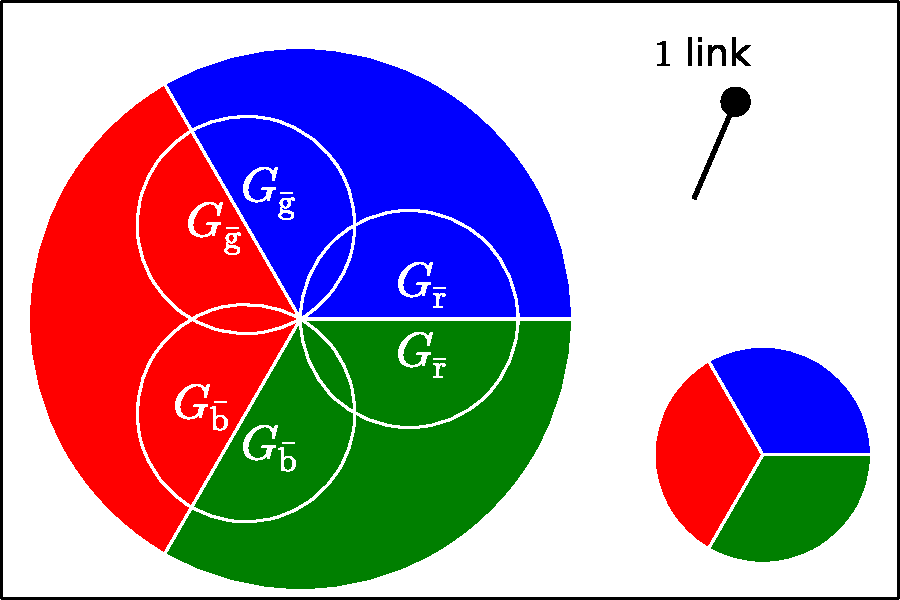
\includegraphics[width=0.2\columnwidth]{sets_1_all.pdf}\qquad
    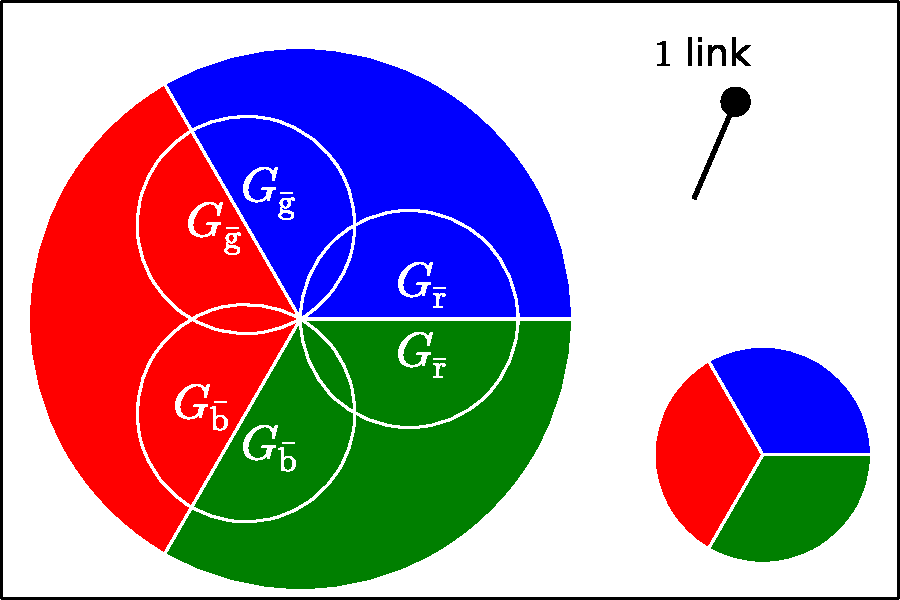
\includegraphics[width=0.2\columnwidth]{sets_1_all.pdf}\qquad
    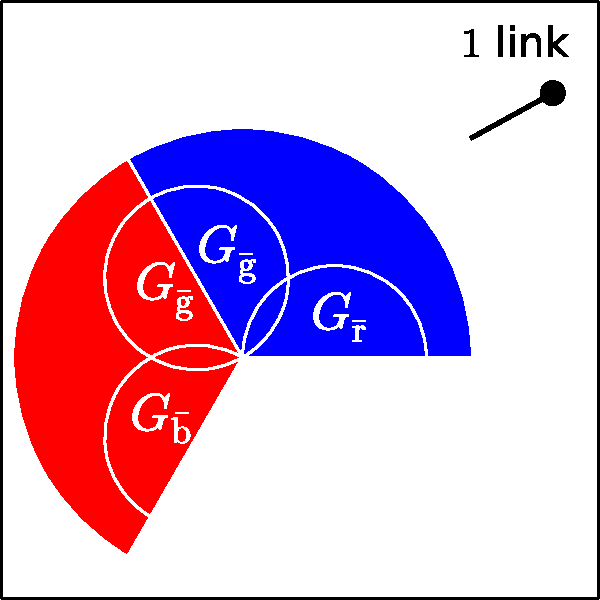
\includegraphics[width=0.2\columnwidth]{sets_1_no_2_gc.pdf}\\
     \vspace{1mm}
      { \hspace{4mm} $\downarrow u$\hspace{36mm}$\downarrow r_{\rm g}$ 
      \hspace{36mm}$\downarrow u_{\bar{\rm g}}$ \hspace{36mm}$\downarrow U_{\bar{\rm g}}$}\\
     \vspace{1mm}
    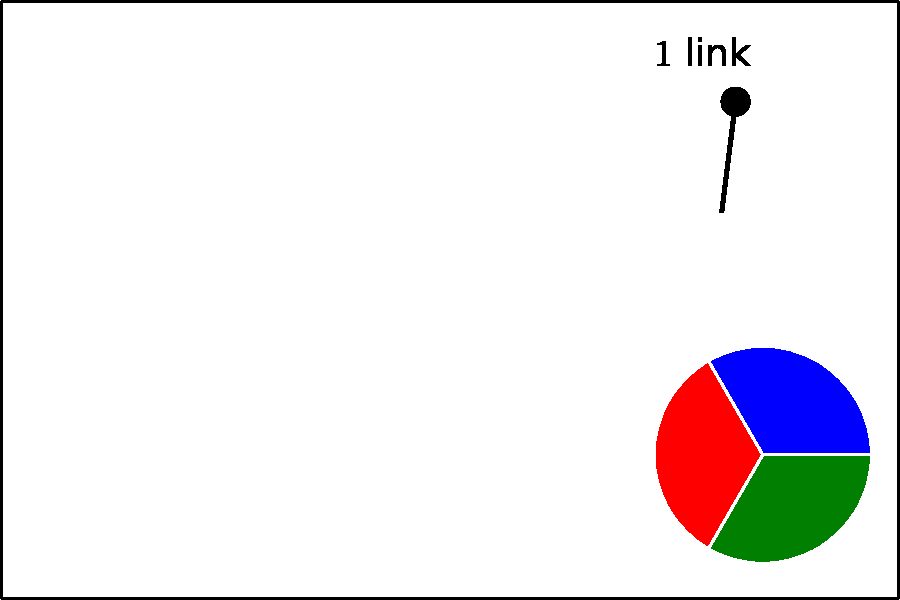
\includegraphics[width=0.2\columnwidth]{sets_1_no_gc.pdf}\qquad
    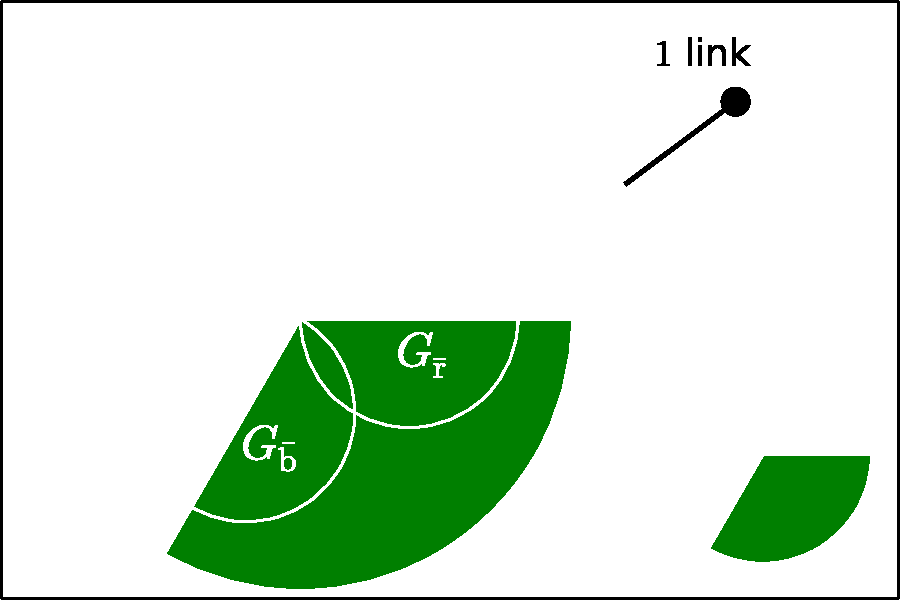
\includegraphics[width=0.2\columnwidth]{sets_1_c2.pdf}\qquad
    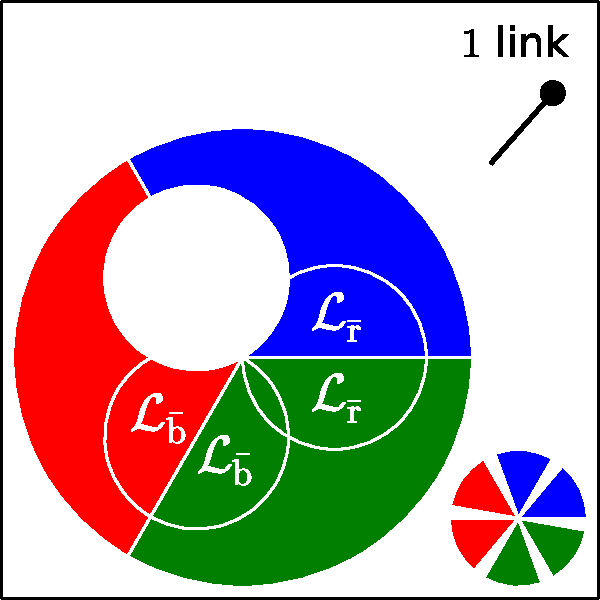
\includegraphics[width=0.2\columnwidth]{sets_1_gc_no_gc_no_2.pdf}\qquad
    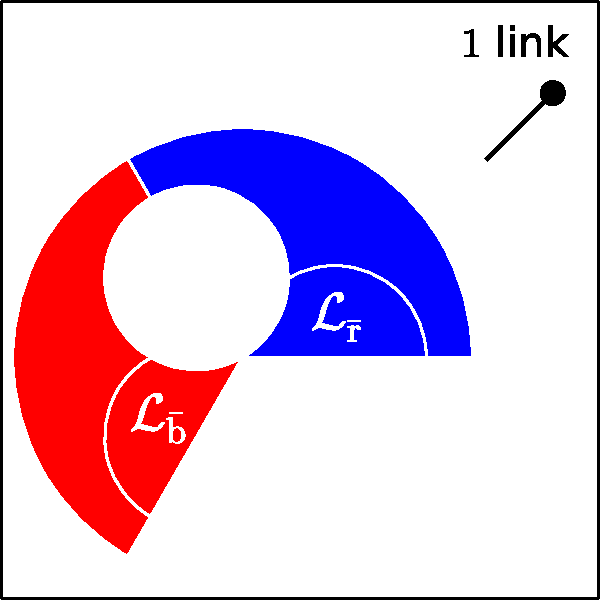
\includegraphics[width=0.2\columnwidth]{sets_1_no_2_gc_no.pdf}
   \end{center}
  \caption{Probabilities for a single link to connect to different parts of the network. We 
  use these probabilities as primitives to calculate the probability for many links. While 
  $u$, $r_c$ and $u_{\bar c}$ can be calculated with standard methods invented for the 
  configuration model before, the conditional probability $U_{\bar c}$ can be calculated as 
  a combination of the others.}
  \label{fig:primitives}
\end{figure}
%
We already gave equation~\ref{eq:u} for calculating the probability $u$. 
In the case of colors on the nodes, as illustrated 
in figure~\ref{fig:primitives} on the left, the colors can simply be ignored. 
We further define $r_c$ as the probability to connect to a node of color $c$. 
This is illustrated in the second column of the figure. 
$r_c$ has to include the fact that high degree nodes are reached more probably, 
therefore the colors on high degree nodes are found with higher probability: 
%%%
\begin{align}
r_c &= \sum_k k p_k {\tilde r}_{c,k}/{\bar k}.\label{eq:r_c}
\end{align}
If ${\tilde r}_{c,k}$ does not depend on the degree $k$, $r_c={\tilde r}_{c,k}$.
We further introduce $u_{\bar c}$, 
the probability that a single link does not connect to a giant $\mathcal{L}_{\bar c}$. 
See the third column of the figure for an illustration. 
This can be calculated using percolation theory 
for degree-dependent (targeted) attack by solving 
%%%
\begin{align}
u_{\bar c} &= 1- f_1(1) +  f_1(u_{\bar c}),\quad 
f_1(z)=\sum_k q_k (1-{\tilde r}_{c,k+1}) z^k.\label{eq:u_c}
\end{align}
Again, if the color distribution is independent of the degree, 
we get the simpler expression 
$u_{\bar c} = r_c + (1-r_c) g_1(u_{\bar c})$ (percolation with random attack). 

\begin{figure}[htb]
  \begin{minipage}[b]{0.2\linewidth}
    \begin{center}
    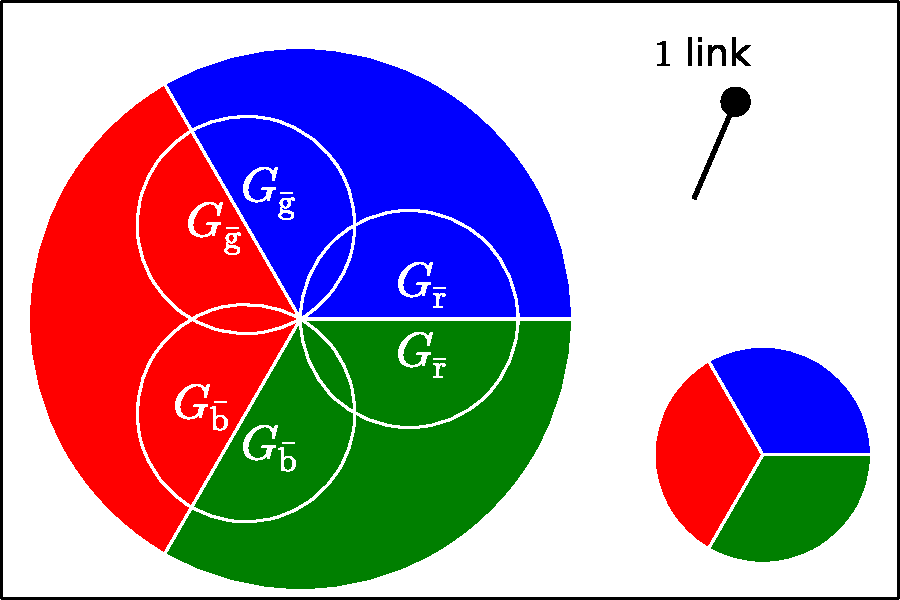
\includegraphics[width=0.99\columnwidth]{sets_1_all.pdf}\\
      \vspace{42mm}
   \end{center}
  \end{minipage}
  \begin{minipage}[b]{0.15\linewidth}
    \begin{center}
      $(1-u)(1-r_{\rm g})$\\
      {\large $\rightarrow$\\}
      \vspace{20mm}
      $1-u_{\bar{\rm g}}$\\
      {\large $\searrow$\\}
      \vspace{27mm}
    \end{center}
  \end{minipage}
  \begin{minipage}[b]{0.2\linewidth}
    \begin{center}
    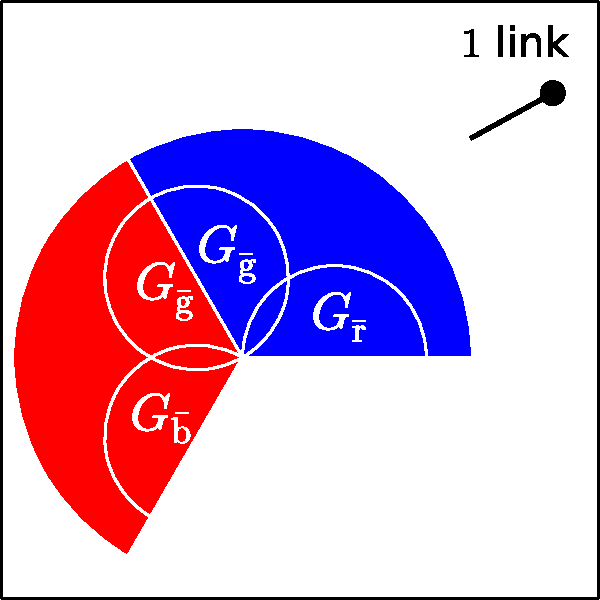
\includegraphics[width=0.99\columnwidth]{sets_1_no_2_gc.pdf}\\
     \vspace{1mm}
    {\large $\downarrow$} $1-U_{\bar{\rm g}}$\\
     \vspace{1mm}
    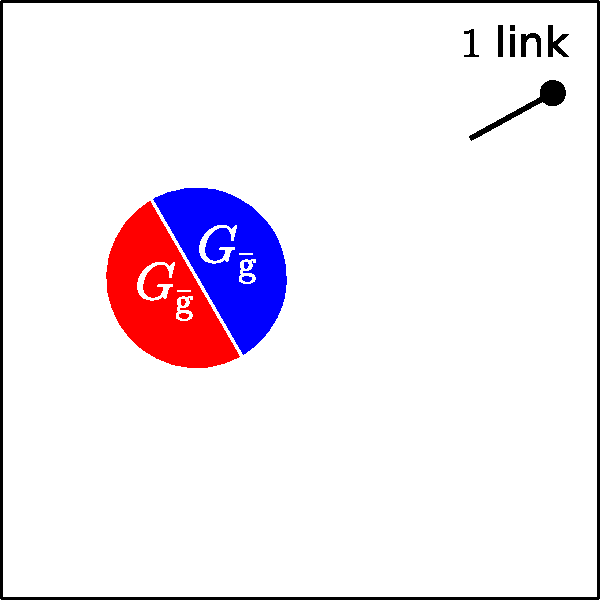
\includegraphics[width=0.99\columnwidth]{sets_1_gc_no_2.pdf}\\
   \end{center}
  \end{minipage}
    \caption{This figure illustrates the calculation of $U_{\bar{\rm g}}$ 
    using the equality $(1-u)(1-r_{\rm g})(1-U_{\bar{\rm g}})=1-u_{\bar{\rm g}}$. For 
    that, we have assumed independence of the qualities of the link under 
    consideration, especially of the color it connects to and if it connects to 
    the giant component. }
    \label{fig:U_c}
\end{figure}
%%%
Unfortunately, $u_{\bar c}$ cannot be used directly for calculating $S_{\rm color}$. 
If we look at the same link, 
the probabilities $u_{\bar c}$ are dependent for different colors. 
The most obvious argument is that always $\Pi_c (1-u_{\bar c})=0$, 
as a link must at least miss one of the $\mathcal{L}_{\bar c}$. 
Instead, we will use the conditional probability $U_{\bar c}$, 
as illustrated with the outer right column of the figure. 
The precondition is that a link connects to the giant component 
and the node it connects to has not color $c$. 
$U_{\bar c}$ is the probability that such a link connects to $\mathcal{L}_{\bar c}$. 
For calculating it, we use the primitives introduced so far, 
as illustrated in figure~\ref{fig:U_c}. 
Assuming independence of the probabilities $(1-u)$ for connecting to the giant component 
and $(1-r_c)$ for not connecting to a node of color $c$, 
the precondition of $U_{\bar c}$ can be constructed. 
In this way, we can construct $(1-u_{\bar c})$ using the probability we are searching for: 
$(1-u_{\bar c}) = (1-u)(1-r_c)(1-U_{\bar c})$. With this we find  
%%%
\begin{align}
U_{\bar c} &= 1 - \frac{1-u_{\bar c}}{(1-u)(1-r_c)}.\label{eq:U_c}
\end{align}
%%%
Notice that the additional information of the explicit color, instead of only stating that the color 
is not $c$, does not alter the results, as a further restriction of the colors 
would meat the numerator and denominator identically and therefore would cancel out. 





\subsection{Averaging over link distributions}




\begin{figure}[htb]
  \begin{minipage}[b]{0.22\linewidth}
    \begin{center}
    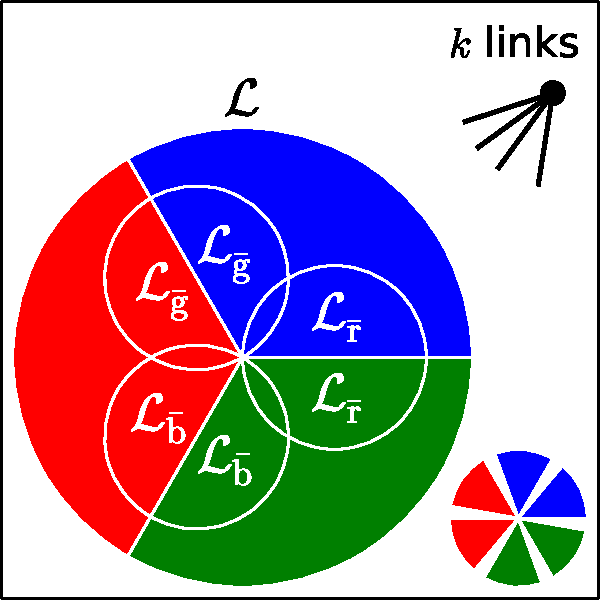
\includegraphics[width=0.99\columnwidth]{sets_k_all.pdf}
   \end{center}
  \end{minipage}
  \begin{minipage}[b]{0.1\linewidth}
    \ 
  \end{minipage}
  \begin{minipage}[b]{0.54\linewidth}
    \begin{center}
    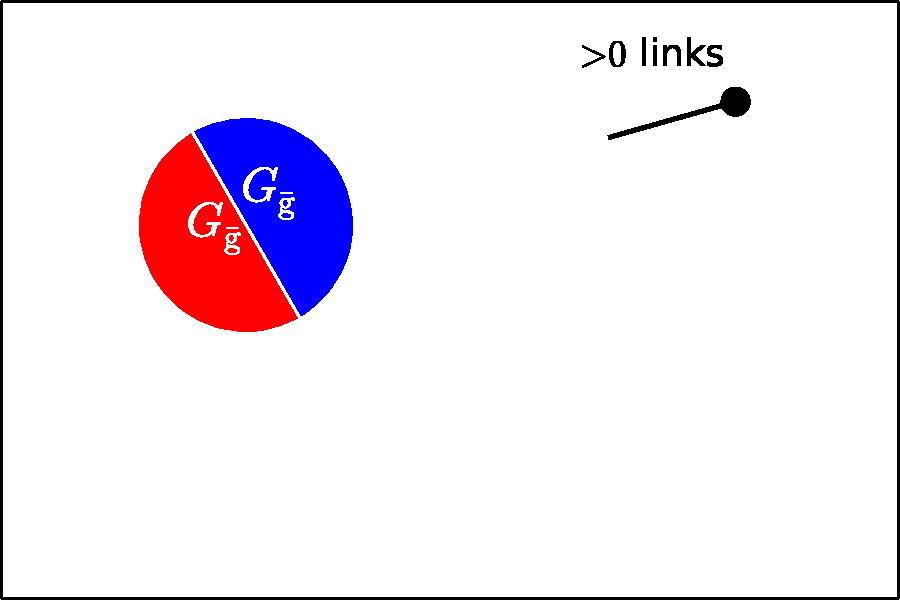
\includegraphics[height=0.4\columnwidth]{sets_k_gc_no_2.pdf}
     \hspace{-1mm}
    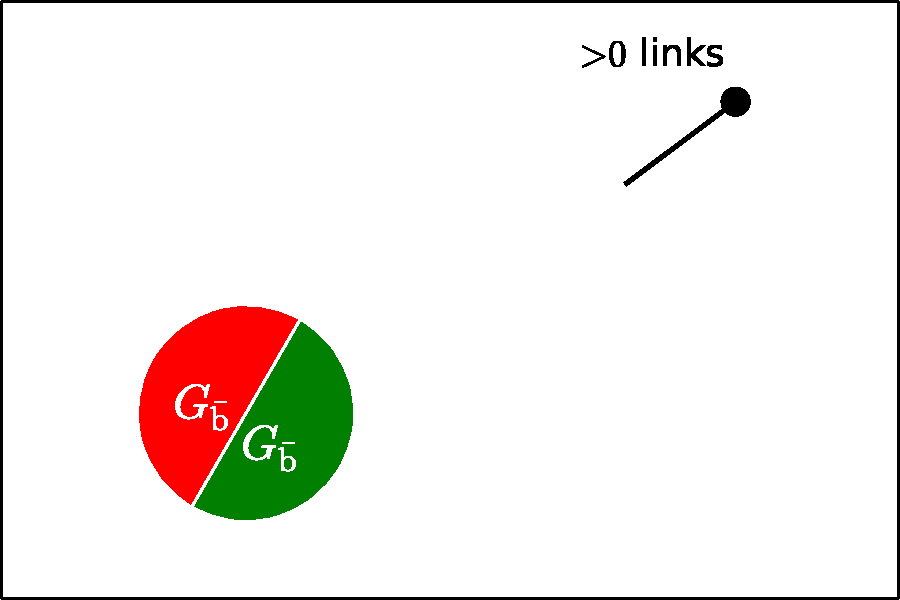
\includegraphics[trim=100 0 0 0,clip,height=0.4\columnwidth]{sets_k_gc_no_3.pdf}
     \hspace{-1mm}
    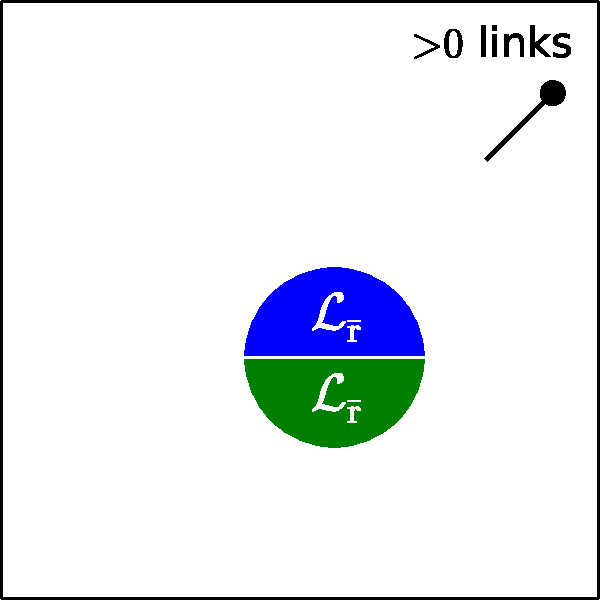
\includegraphics[trim=100 0 0 0,clip,height=0.4\columnwidth]{sets_k_gc_no_1.pdf}
   \end{center}
  \end{minipage}\\
     \vspace{2mm}
      {\large \hspace{-30mm} $\downarrow B_{k,k'}$\hspace{90mm}$\uparrow P_{\vec \kappa}$ }\\
     \vspace{2mm}
  \begin{minipage}[b]{0.22\linewidth}
    \begin{center}
    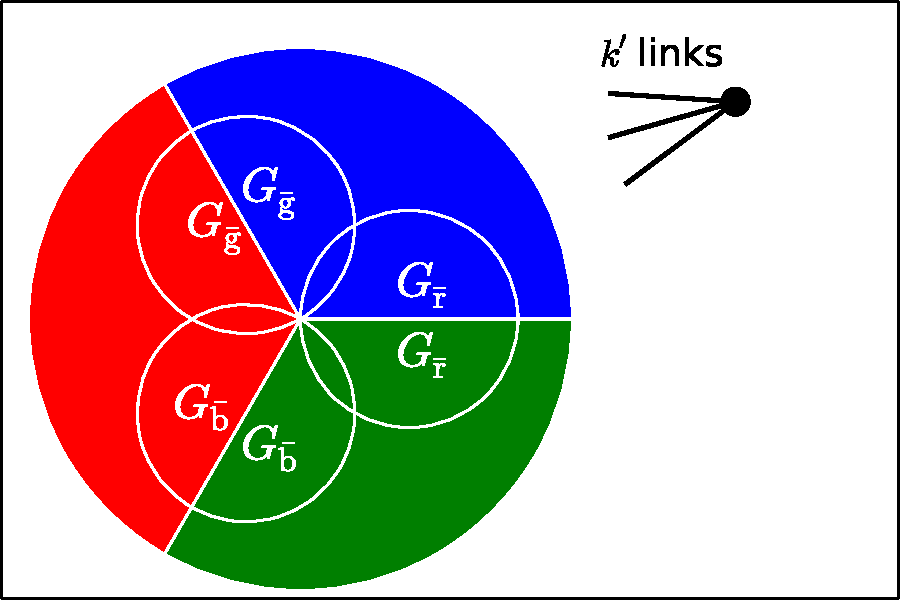
\includegraphics[width=0.99\columnwidth]{sets_k_gc.pdf}
   \end{center}
  \end{minipage}
  \begin{minipage}[b]{0.1\linewidth}
    \begin{center}
      {\Large $\xrightarrow{M_{k',\vec{\kappa}}}$}\\
      \vspace{20mm}
    \end{center}
  \end{minipage}
  \begin{minipage}[b]{0.54\linewidth}
    \begin{center}
    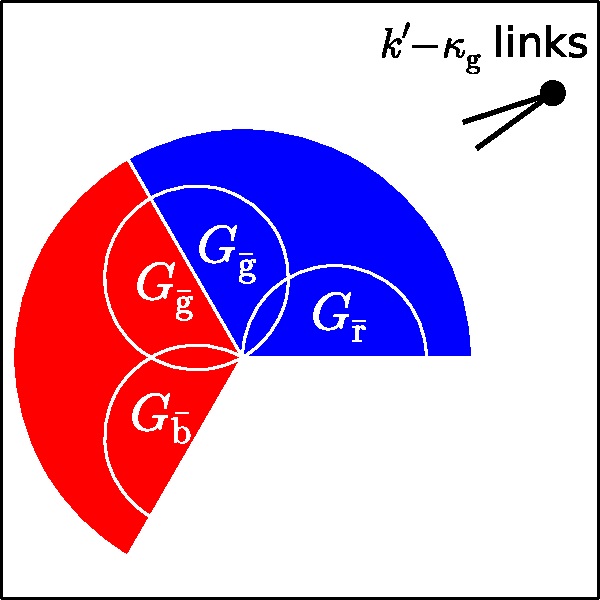
\includegraphics[height=0.4\columnwidth]{sets_k_no_2_gc.pdf}
     \hspace{-1mm}
    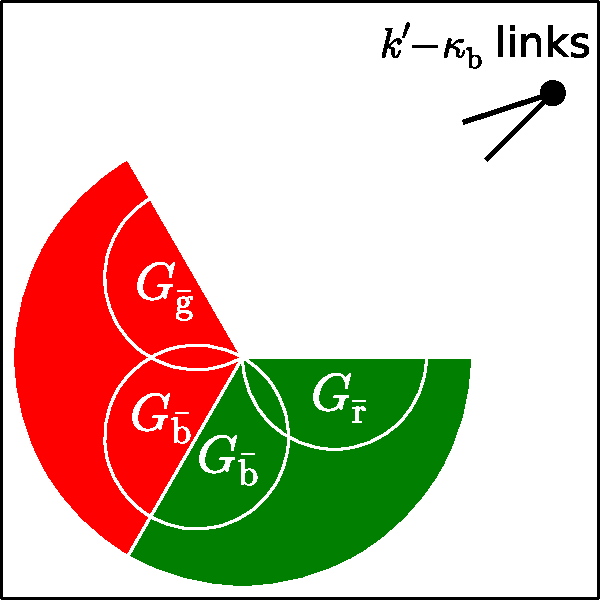
\includegraphics[trim=100 0 0 0,clip,height=0.4\columnwidth]{sets_k_no_3_gc.pdf}
     \hspace{-1mm}
    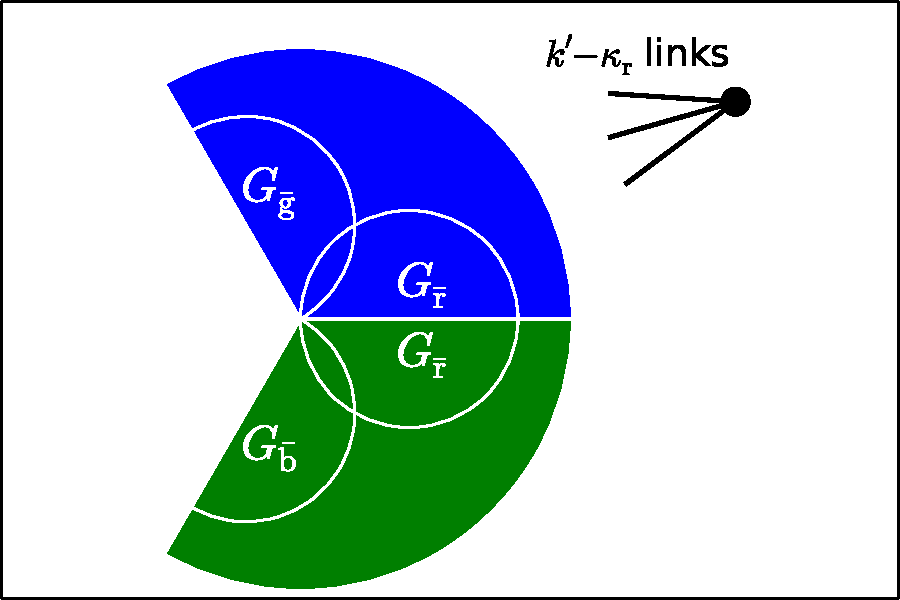
\includegraphics[trim=100 0 0 0,clip,height=0.4\columnwidth]{sets_k_no_1_gc.pdf}
   \end{center}
  \end{minipage}
    \caption{For calculating the probability of a node with $k$ links to belong to 
    $\mathcal{L}_{\rm color}$, we have to average over different link constellations which this node 
    might show. First, $B_{k,k'}$ is the probability that out of the $k$ links $k'$ 
    connect to the giant component. It is calculated using $u$ (compare figure~\ref{fig:primitives} 
    on the left). Second, $M_{k',\vec{\kappa}}$ gives the probability for a certain color 
    distribution among the links. It is calculated using $r_{\rm g}$ etc. (compare 
    figure~\ref{fig:primitives}, second from left). We assume that this second step is 
    independent of the first step, what is confirmed with the final results. Third, 
    $P_{\vec \kappa}$ gives the joint probability that for this color distribution 
    $\mathcal{L}_{\bar{\rm r}}$, $\mathcal{L}_{\bar{\rm b}}$ and $\mathcal{L}_{\bar{\rm g}}$ are connected to at 
    the same time. This is calculated using $U_{\bar{\rm r}}$ etc. (compare 
    figure~\ref{fig:primitives} on the right).}
    \label{fig:stepwise}
\end{figure}
%%%
As in equation~\ref{eq:S} for the giant component, 
we want to get an analytical result for $S_{\rm color}$ 
by averaging over possible link constellations of a randomly chosen node. 
Let us give the whole result and then explain it step by step afterwards:
%%%
\begin{align}
S_{\rm color} &= \sum_{k=0}^{\infty}p_k \sum_{k'=0}^{k} B_{k,k'} 
\sum_{\kappa_1,\dots, \kappa_C=0}^{k'} M_{k',\vec \kappa} 
P_{\vec \kappa},\label{eq:S_color}\\
B_{k,k'} &={k \choose k'}(1-u)^{k'}u^{k-k'},\label{eq:B}\\
M_{k',\vec \kappa} &=\frac{k'!}{\kappa_1! \times \dots \times \kappa_C!} \,
(r_1)^{\kappa_1} \times \dots \times (r_C)^{\kappa_C}\,
\delta_{k',\kappa_1+\dots + \kappa_C},\\
P_{\vec \kappa} &= \prod_{c=1}^C [1-(U_{\bar c})^{k'- \kappa_c }].\label{eq:p_success}
\end{align}
The formulas include the single link probabilities $u$, $r_c$ and $U_{\bar C}$ 
of equations~\eqref{eq:u},~\eqref{eq:r_c}~and~\eqref{eq:U_c} (the last depends on~\eqref{eq:u_c}). 
An illustration of the procedure can be seen in figure~\ref{fig:stepwise}.
$B_{k,k'}$ is the binomial probability that out of the $k$ links $k'$ links connect to the giant component. 
$M_{k',\vec{\kappa}}$ gives the multinomial probability 
for a certain color distribution among the $k'$ links connecting to the giant component.
We assume that this second step is independent of the first step, 
what is confirmed with the final results. 
The numbers $\kappa_c$ count the links which connect to a node of color $c$ in the giant component. 
Finally, $P_{\vec \kappa}$ gives the joint probability 
that for the color distribution given by $\vec \kappa$ 
all giant $\mathcal{L}_{\bar c}$ are connected to at the same time. 
There is at least one link connecting to ${\mathcal L}_{\bar c}$ 
with probability $1-(U_{\bar c})^{k' - \kappa_c }$. 
The success probabilities for different colors have to be multiplied, 
as all ${\mathcal L}_{\bar c}$ have to be reached at the same time. 
We tested numerically that e.g. $U_{\bar{\rm 1}}$ and $U_{\bar{\rm 2}}$ are independent for a link 
connecting to the giant component and a third color. 




\section{Examination of the theory}


\subsection{$k'$-decomposition and an upper bound}

For a further examination of $S_{\rm color}$, 
it is useful to rearrange equation~\ref{eq:S_color} with focus on $k'$, 
the number of links connecting a single randomly chosen node to the giant component, 
\begin{align}
S_{\rm color} &= \sum_{k'=0}^{\infty} \underbrace{\sum_{k=k'}^{\infty} p_k B_{k,k'}}_{\pi_{k'}}
\underbrace{{\sum_{\kappa_1,\dots=0}^1 M_{k',\vec \kappa} P_{\vec \kappa}}}_{\sigma_{k'}}
 = \sum_{k'=0}^{\infty} \pi_{k'}\sigma_{k'}.
\end{align}
The first term $\pi_{k'}$ gives the probability that a randomly chosen node 
connects over exactly $k'$ nodes to the giant component. 
Using equation~\ref{eq:B}, it can be shown that $\sum_{k'=0}^{\infty}\pi_{k'}=1$. 
This quality is meaningful, as every link should have 
either no or some connections to the giant component. 
Using the same equation, we can write $\pi_{k'}$ in terms of generating functions, 
\begin{align}
\pi_{k'} &= \frac{(1-u)^{k'}}{k'!}\left.\frac{{\rm d}^{k'}g_0(z)}{{\rm d}z^{k'}}\right|_{z=u}.
\end{align}
By construction of the generating function we have $\pi_{k'}=p_k$ for $u=0$, 
what should hold of cause. 
With equation~\ref{eq:S} we find $S=1-\pi_0=\sum_{k'=1}^{\infty}\pi_{k'}$. 

The second term $\sigma_{k'}$ is the probability that a node 
connecting over $k'$ links to the giant component belongs to $S_{\rm color}$. 
As can be seen with equation~\ref{eq:p_success}, $\sigma_0=\sigma_1=0$. 
On the other hand, with $k'\geq 2$ and probabilities $U_{\bar c}$ close to zero, 
$\sigma_{k'}\leq 1$ can come close to its upper limit. 
Therefore the upper limit 
\begin{align}
S_{\rm color}\leq \sum_{k'=2}^{\infty} \pi_{k'} = 1-\pi_0-\pi_1 &\equiv S_{\rm color,\infty} 
\end{align}
is useful. Compared to the size of the giant component $S=1-\pi_0$, 
$S_{\rm color}$ misses at least all nodes 
which are connected to the giant component over $k'=1$ links. 
This result is closely connected to $k$-core percolation with $k=2$. 
Note that $k$-core percolation shows a continuous phase transition for $k=2$, 
and only for $k>2$ has the well known discontinuous behavior. 


\subsection{Closed form solutions}

\begin{figure}[htb]
    \includegraphics[width=0.49\columnwidth]{cross_over_2.pdf}\\
    \caption{$S_{\rm color}$ can be divided into contributions of nodes with different numbers 
    $k'$ of links to the giant component.}
    \label{fig:2_colors}
\end{figure}
%
We now will calculate a closed form result for $S_{\rm color}$ 
on Poisson graphs with two colors. 
This is done to demonstrate how the extensive summations 
over $k'$, $k$ and $\vec \kappa$ can be performed analytically. 
In cases where this is not possible, 
a sampling of values $\vec \kappa$ has to be performed. 
The results can be tested against the analytically tractable situations 
and by comparing with numerical results. 
Additionally, our result will help us to gain first insights about the critical behavior. 

For Poisson graphs, $\pi_{k'}$ can be given in a short and useful form for all $k'$. 
Instead of using generating functions, we simply rewrite 
\begin{align}
\pi_{k'} &= \sum_{k=k'}^{\infty} \frac{{\bar k}^k e^{-{\bar k}}}{k!} \frac{k!}{(k-k')!k'!}u^{k-k'}(1-u)^{k'}\\
 &= \underbrace{ \frac{{\bar k}^{k'} e^{-{\bar k}}}{k'!}}_{p_{k'}} e^{u \bar k} (1-u)^{k'}
 \underbrace{ \sum_{k=k'}^{\infty} \frac{({u\bar k})^{k-k'} e^{-{u\bar k}}}{(k-k')!}}_{1}\\
 &= p_{k'} e^{u \bar k} (1-u)^{k'}.
\end{align}
The most promising fact of this result is that it contains $p_{k'}$, 
and therefor the simply evaluable generating function of the Poisson distribution can be used below, 
\begin{align}
g_0(z) &= e^{\bar{k}(z-1)}.\label{eq:g0}
\end{align}


For evaluating $\sigma_{k'}$ with two colors, we rewrite 
\begin{align}
\sigma_{k'} &= \sum_{\kappa_1=0}^{k'} {k' \choose \kappa_1}\, 
(r_1)^{\kappa_1} (r_2)^{k'-\kappa_1}\,
[1-(U_{\bar 1})^{k'-\kappa_1 }] [1-(U_{\bar 2})^{\kappa_1 }]\\
&= \sum_{\kappa_1=0}^{k'} {k' \choose \kappa_1}\, 
\left[
(r_1)^{\kappa_1} (r_2)^{k'-\kappa_1}\, - 
(r_1 U_{\bar 2})^{\kappa_1} (r_2)^{k'-\kappa_1}\,-
(r_1)^{\kappa_1} (r_2 U_{\bar 1})^{k'-\kappa_1}\,+
(r_1 U_{\bar 2})^{\kappa_1} (r_2 U_{\bar 1})^{k'-\kappa_1}]
\right]\\
 &= 1 - (r_1+r_2 U_{\bar 1})^{k'} - (r_2+r_1 U_{\bar 2})^{k'} + (r_1 U_{\bar 2} + r_2 U_{\bar 1})^{k'}.
\end{align}
In the last step, the binomial formula was used backward. 
Notice that this result is independent of the degree distribution. 
In figure~\ref{fig:2_colors}, $\sigma_{k'}$ (upper panel), 
$\pi_{k'}$ (lower panel with dashed lines) and $\sigma_{k'}\pi_{k'}$ (solid lines)
are given for $k'=2$ (blue), $k'=4$ (red) and $k'=7$ (green) on Poisson graphs. 
The fat black line shows $S_{\rm color}$. 
We continue with the Poisson distribution and find with equation~\ref{eq:U_c} and some rewriting 
\begin{align}
S_{\rm color} &= e^{u \bar{k}} \sum_{k'=0}^{\infty} p_{k'} (1-u)^{k'}\sigma_{k'}\\
 &= e^{u \bar{k}} [g_0(1-u) - g_0(u_{\bar 1} -u) - 
g_0(u_{\bar 2} -u) + g_0(u_{\bar 1} + u_{\bar 2} -1-u)].
\end{align}
For larger numbers of colors, giant $\mathcal{L}_{\bar c}$ will overlap. 
This is reflected in terms including products of the conditional probabilities $U_{\bar c}$ 
which cannot be further simplified. 
However, even for larger numbers of colors 
there are closed form expressions with generating functions. 
They contain increasing numbers of terms for increasing $C$, 
therefore they are probably only useful for a few colors. 
For two colors, it is even possible to rewrite the final result as a simple product: 
\begin{align}
S_{\rm color} &= [1-g_0(u_{\bar 1})] [1-g_0(u_{\bar 2})].\label{eq:2_colors}
\end{align}



\subsection{Critical behavior for Poisson graphs}

The terms $\sigma_{k'}$ imply demanding summations and products, 
and the critical behavior will be evaluated with a number of consecutive approximations. 
For give a first glance, it is useful to discuss the case with two colors first. 
For this we found a simple closed form expression 
which can be discussed without much effort. 

\subsubsection{Two colors}

With equations~\eqref{eq:u_c},~\eqref{eq:g0} and~\eqref{eq:2_colors} we have to analyze 
\begin{align}
S_{\rm color} &= [1-g_0(u_{\bar 1})] [1-g_0(u_{\bar 2})],\\
u_{\bar c} &= r_c+(1-r_c) g_1(u_{\bar c}).
\end{align}




\subsubsection{Critical connectivity with homogeneous color distribution}

As long as $U_{\bar c}=1$ for any color $c$, 
$P_{\vec \kappa} = \prod_{c=1}^C [1-(U_{\bar c})^{k'- \kappa_{c} }]$ 
vanishes, and therefore $\sigma_{k'}=0$ for every $k'$. For a homogeneous color 
distribution we have $r_c=r_1=1/C$ for all colors $c$, and accordingly 
$U_{\bar c}=U_{\bar 1}$ is identical for all colors. As for $\bar{k}\leq 1$ the 
giant component has vanishing size, the conditional probability 
\begin{align}
U_{\bar 1} &= 1 - \frac{1-u_{\bar 1}}{(1-u)(1-r_1)}
\end{align}
is not defined in this region. However, we find $S_{\rm color}=0$ due to $\pi_{k'}=0$. 
For $\bar{k}>1$, $U_{\bar c}=1$ whenever $u_{\bar 1}=1$, meaning that a single link has vanishing 
probability to connect to $G_{\bar 1}$. We can find 
\begin{align}
u_{\bar 1}(\bar{k}) &= r_1 - (1-r_1)u[\bar{k}(1-r_1)],\label{eq:u_1_solution}
\end{align}
as this solution inserted into the self consistency equation $u_{\bar 1}=r_1+(1-r_1)g_1(u_{\bar 1})$
leads to the self consistency equation of $u=g_1(u)$. This enables us to calculate the critical 
value $\bar{k}_{\rm crit}$, below which $S_{\rm color}=0$: 
\begin{align}
{\bar k}_{\rm crit} &= 1/(1-r_1) = C/(C-1).
\end{align}



\subsubsection{Critical behavior for a few colors}

The normal giant component size $S$ shows a special critical behavior shortly above the transition point, 
it scales linearly with $\bar{k}-1$. Here we are interested in the behavior of $S_{\rm color}$ 
which is a function of $1-u_{\bar 1}$ which itself can be related to $1-u=S$. For small arguments
$(\bar{k}-{\bar k}_{\rm crit})$, 
\begin{align}
1-u_{\bar 1}(\bar{k}>{\bar k}_{\rm crit}) &\approx 
(1-r_1)^2 \left.\frac{{\rm d}(1-u)}{{\rm d}{\bar k}}\right|_{\bar{k}=1+0} (\bar{k}-{\bar k}_{\rm crit})
\end{align}
holds due to equation~\ref{eq:u_1_solution}. Inserting into $U_{\bar 1}$ we find using 
$1-u(\bar{k}>1) \approx \left.\frac{{\rm d}(1-u)}{{\rm d}{\bar k}}\right|_{\bar{k}=1+0} (\bar{k}-1)$
\begin{align}
\varepsilon &\equiv 1 - U_{\bar 1} \approx C (\bar{k}-{\bar k}_{\rm crit})
\end{align}
if additionally $\bar{k}-{\bar k}_{\rm crit}\ll\bar{k}-1$ holds ($1-u_{\bar 1}$ small compared to 
$1-u$). 

For calculating $\sigma_{k'}$, we first need to evaluate $P_{\vec \kappa}$ including expressions 
$1-(U_{\bar 1})^{k'-\kappa_c}$. Replacing with $\varepsilon$ and applying an approximation we find 
$1-(U_{\bar 1})^{k'-\kappa_c}=1-(1-\varepsilon)^{k'-\kappa_c}\approx (k'-\kappa_c) \varepsilon$. 
This is true at least as long as $k'\varepsilon\ll 1$. With this we find 
$P_{\vec \kappa}\propto (\bar{k}-{\bar k}_{\rm crit})^C$ independent of $\vec \kappa$, and finally 
\begin{align}
\sigma_{k'} &\propto (\bar{k}-{\bar k}_{\rm crit})^C. 
\end{align}
We will see below that the largest $k'$ giving a notable contribution to $S_{\rm color}$ is 
smaller then the number of colors $C$, therefore $k'\varepsilon\ll 1$ can be met and we finally find 
\begin{align}
S_{\rm color} &\propto (\bar{k}-{\bar k}_{\rm crit})^{\beta},\\
\beta &= C.
\end{align}



\subsubsection{Staircase of crossovers for many colors}

\begin{figure}[htb]
    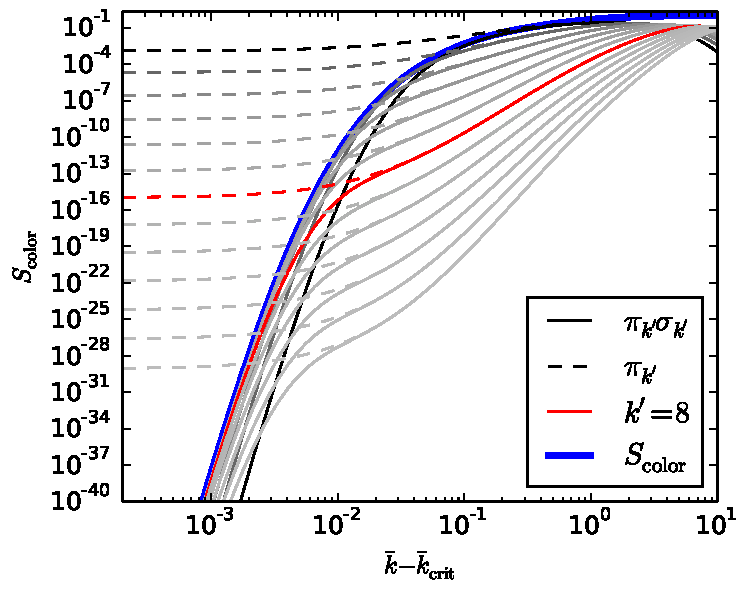
\includegraphics[width=0.49\columnwidth]{cross_over_C40.pdf}
    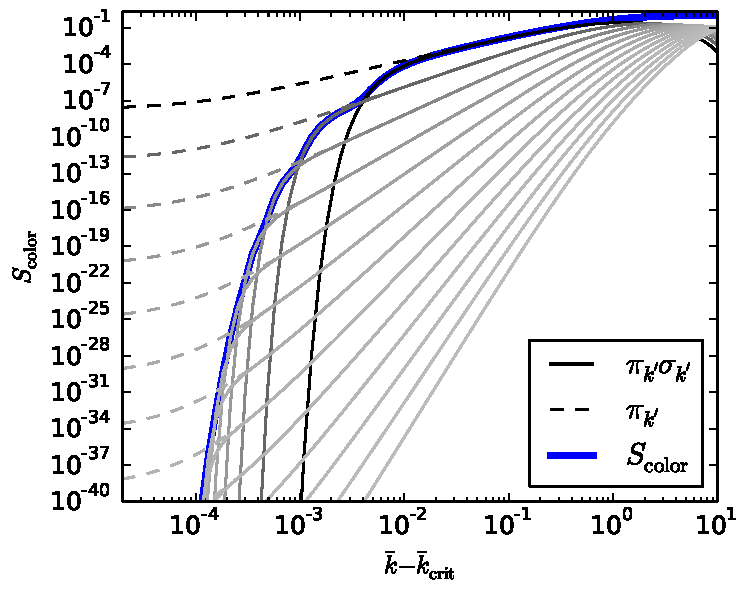
\includegraphics[width=0.49\columnwidth]{cross_over_C10000.pdf}\\
    \caption{$S_{\rm color}$ can be divided into contributions of nodes with different numbers 
    $k'$ of links to the giant component.}
    \label{fig:1}
\end{figure}
%
For large numbers of colors $C$, the functions $\sigma_{k'}$ have a rather extreme scaling 
behavior $\sigma_{k'} \propto (\bar{k}-{\bar k}_{\rm crit})^C$. This causes two open 
questions. First, as the functions $\sigma_{k'}$ are saturating to one for high 
values of $\bar{k}-{\bar k}_{\rm crit}$, there could be almost jump-like behavior. 
Second, contributions with increasing $k'$ become important. Roughly speaking, this is due 
to the fact that $\sigma_{k'}$ is going to zero very fast with $\bar{k}-{\bar k}_{\rm crit}\to 0$, 
and therefore the exponential suppression in $\pi_{k'}$ with $k'$ is compensated for. 

For attacking both of these questions, let us apply an approximation. With a homogeneous color 
distribution $U_{\bar c}=U_{\bar 1}$ and an expected value $\left<\kappa_c \right>=k'/C \ll k'$, 
we find
\begin{align}
P_{\vec \kappa} &\stackrel{<}{\approx} (1-(U_{\bar 1})^{k'})^C,\\
\sigma_{k'} &\stackrel{<}{\approx} (1-(U_{\bar 1})^{k'})^C.
\end{align}
As the approximate $P_{\vec \kappa}$ is independent of $\vec \kappa$, the summation over $M_{k',\vec \kappa}$ was 
easily executed. Now we are able to compare the contributions $\pi_{k'}\sigma_{k'}$ for 
$\bar{k}\to \bar{k}_{\rm crit}$, implying that $k'\varepsilon\ll 1$ holds. We have to find, whether above a 
certain $k'$ the following holds:
\begin{align}
\log(\frac{\pi_{k'+1}\sigma_{k'+1}}{\pi_{k'}\sigma_{k'}}) &< 0.
\end{align}
We can find with 
\begin{align}
\log(\sigma_{k'})&\approx C \log[k' (1-u_{\bar 1})/((1-u)(1-r_1)]\\
&\approx C\log(k') +\{{\rm independent\, of\,} k'\},\\
\log(\pi_{k'}) &= k' \log(\bar{k}) - \log(k'!)+k'\log(1-u) +\{{\rm independent\, of\,} k'\}.\\
\end{align}
and using $\log(\bar{k}_{\rm crit})\approx 1/C$ and $\log(1-u(\bar{k}_{\rm crit}))\approx -\log(C)$ 
and $\log(1=x)\approx x$ for small $x$:
\begin{align}
\log(\frac{\pi_{k'+1}\sigma_{k'+1}}{\pi_{k'}\sigma_{k'}}) &\approx C/k' - \log(k') +1/C -\log(C).\\
\end{align}
This falls below zero approximately at $k'\log(Ck')=C$, and clearly contributions are exponentially 
dampened with large $k'$. Up to the $k'$ with $k'\log(Ck')=C$, contributions $\pi_{k'}\sigma_{k'}$ 
grow. That is surprising, as nodes with increasing $k'$ should be much less probable. However, 
if $\sigma_{k'}$ is very small that compensates for the other effect in a certain regime of $k'$. 
For estimating the critical region, where $S_{\rm color}\propto (\bar{k}-{\bar k}_{\rm crit})^C$, we 
use the upper bound for the leading term $k'=C$ and find with 
$k'\varepsilon=k'C (\bar{k}-{\bar k}_{\rm crit})\ll1$ finally 
\begin{align}
(\bar{k}-{\bar k}_{\rm crit}) &\ll 1/C^2.
\end{align}
This region is not of practical importance for large $C$, as there are very small values 
$S_{\rm color}$. 




\pagebreak


Notice that this expression does not depend on $\vec \kappa$, what allows us to evaluate 
the summation over $M_{k',\vec \kappa}$ with result one. We have 
\begin{align}
S_{\rm color} &\leq \sum_{k'=2}^{\infty} \pi_{k'} \sigma_{k'}.
\end{align}
We will show below that $\sigma_{k'}$ has the following shape: 
\begin{align}
\sigma_{k'} &\approx
\begin{cases}
0 & {\bar k} < {\bar k}_{\rm crit}\\
a ({\bar k}-{\bar k}_{\rm crit})^C & {\bar k}_{\rm crit} < {\bar k} \ll {\bar k}_{\rm sat} \\
1 & {\bar k}_{\rm sat} \ll {\bar k}
\end{cases},\\
{\bar k}_{\rm crit} &= 1/(1-r_1) = C/(C-1),\\
a_{k'} &= \dots\\
{\bar k}_{\rm sat}(k') &= C^{-(k'-1)/{k'}}*(1-C^{-1/k'}).\\
\end{align}



Below 
${\bar k}_{\rm crit} = 1/(1-r_1) = C/(C-1)$ it is zero (links connected to 
the giant component can not communicate with avoidable colors). Above the critical value 
${\bar k}_{\rm crit}$, the critical behavior $\sigma_{k'}\propto ({\bar k}-{\bar k}_{\rm crit})^C$ 
can be observed up to a saturation region. Independent of $k'$, $\sigma_{k'}$ saturates to one, 
however, the argument $\bar k$ where saturation is reached depends on $k'$. We need to calculate 
the saturation regions before combining our results into the total critical behavior. 


\subsubsection{Evaluation of the saturation function}



$U_{\bar 1}(\bar k)$ is a monotone decreasing function with values in the interval 
$[0,1]$

\begin{align}
\sigma_{k'} &\leq (1-(U_{\bar 1})^{k'})^C,\\
U_{\bar 1} &= 1 - \frac{1-u_{\bar 1}}{(1-u)(1-r_1)}
\end{align}

This includes results of the self consistency equations $u=g_1(u)$ and 
$u_{\bar 1}=r_1+(1-r_1)g_1(u_{\bar 1})$ (with $r_1=1/C$).
We can find the critical onset by expanding $g_1(x)=\exp[(x-1){\bar k}]$ for arguments $x\approx 1$: 
\begin{align}
u &\approx a \times ({\bar k}-1)\\
u_{\bar 1} &\approx a (1-r_1)\times ({\bar k}-{\bar k}_{\rm crit})\\
{\bar k}_{\rm crit} &= 1/(1-r_1) = C/(C-1)
\end{align}
with a constant $a$.








\subsection{Critical behavior for Poisson graphs}

With general color distributions $r_c$ ($\sum_c r_c =1$), the color with the largest probability 
$r_c$ dominates 
the behavior, as it corresponds to the largest conditional link failure probability $U_{\bar c}$
in equation~\ref{eq:p_success}. For Poisson graphs, $U_{\bar c}$ 
falls below one at ${\bar k}=1/(1-r_c)$, and as long as one $U_{\bar c}$ is one, equation~\ref{eq:p_success}
gives always zero. Therefor the critical value is 
\begin{align}
{\bar k}_{\rm crit}=1/(1-\max_c r_c).
\end{align}

We can understand the critical exponent with expanding equation~\ref{eq:p_success} using 
$U_{\bar c}=1-\varepsilon$ for the highest color frequency. 
We will show below using results from standard percolation that 
$\varepsilon\propto ({\bar k}-{\bar k}_{\rm crit})$. First of all, we have 
$(U_{\bar c})^{\sum_{c'\neq c} \kappa_{c'} }\approx 1-({\sum_{c'\neq c} \kappa_{c'} })\times \varepsilon$, and therefore we find 
$P_{\vec \kappa} \propto \varepsilon^{n_{\rm deg}}$ (unless $P_{\vec \kappa} = 0$ in the case ${\sum_{c'\neq c} \kappa_{c'} }=0$
for any $c$). As equation~\ref{eq:s_color} is therefore a superposition of either vanishing terms or terms with 
leading order $\varepsilon^{n_{\rm deg}}$, we have 
%%%
\begin{align}
\beta=n_{\rm deg}.
\end{align}
%%%
To complete the discussion of the critical behavior, we have to show that 
$1- U_{\bar c}\propto ({\bar k}-{\bar k}_{\rm crit})$ for a certain region of critical behavior. 
We know from standard percolation theory for Poisson graphs that $S \propto ({\bar k}-1)^1$, and therefore 
$1-u({\bar k})\approx a \times ({\bar k}-1)$ for $\bar k$ exceeding the critical value 
about small values. With inserting into equation~\ref{eq:u_c} it can be shown that 
$u_{\bar c}({\bar k})=1-\phi_{\bar c}+\phi_{\bar c}u({\bar k}\phi)$. Using this in 
equation~\ref{eq:U_c} ($\phi_{\bar c}=1-r_c$), we find 
%%%
\begin{align}
U_{\bar c} &= 1 - \frac{1-u({\bar k}\phi_{\bar c})}{1-u({\bar k})}\\
&\approx 1- \phi_{\bar c} \frac{{\bar k}-{\bar k}_{\rm crit}}{{\bar k}-1}
\end{align}
%%%
which drops linearly from one in the critical region
%%%
\begin{align}
0< {\bar k}-{\bar k}_{\rm crit} &\ll {\bar k}_{\rm crit}-1.
\end{align}
%%%
In figure~\ref{fig:pt} we have ${\bar k}_{\rm crit}-1=1/2$, and critical behavior up to 
about ${\bar k}-{\bar k}_{\rm crit}=1/10$.

As a final remark let us discuss the critical behavior for largest color frequencies which 
are not perfectly degenerated. Lets assume two colors with close by values 
${\bar k}_1< {\bar k}_2$, where $U_{\bar c}$ drops below one. With equation~\ref{eq:p_success} and the definition 
$\varepsilon={\bar k}-{\bar k}_2$ we have above ${\bar k}_2$ that 
$P_{\vec \kappa} \propto \varepsilon \times (\varepsilon+({\bar k}_2 - {\bar k}_1))$. This 
is dominated by a linear term for small $\varepsilon$ and by a quadratic term for larger 
values, the crossover is at about
%%%
\begin{align}
{\bar k}-{\bar k}_2 &= {\bar k}_2-{\bar k}_1.
\end{align}
%%%
Exceeding the critical value ${\bar k}_{\rm crit}={\bar k}_2$ about more than the 
distance ${\bar k}_2 - {\bar k}_1$, $S_{\rm color}$ behaves as 
if the color frequencies would be degenerated. 

With these results altogether we can understand the behavior of $S_{\rm color}$ 
for small frequencies of all colors. There is a deviation 
from $S_{{\rm color},\infty}$ due to $S_{\rm color}=0$ below ${\bar k}_{\rm crit}$, and 
above there is a region of slow critical growth with large critical exponent $\beta$. This region acts as an effective 
shift of the critical parameter. Further increasing $\bar k$, $U_{\bar c}$ saturates smoothly to zero for all colors. 
Accordingly, $S_{\rm color}$ has a smooth rise to finite values, but not governed by a certain critical exponent. 
It comes closer to $S_{{\rm color},\infty}$ without reaching it, as there are other effects (e.g. nodes with 
exactly two links can connect to two nodes of the same color). The smaller the highest color frequencies are, 
the closer $S_{\rm color}$ is to $S_{{\rm color},\infty}$.



%\clearpage


\bibliographystyle{apsrev4-1}
\bibliography{mp}

\end{document}
